\documentclass[runningheads]{llncs}
\usepackage{url}
\usepackage{graphicx}
\usepackage{subfigure}
\usepackage[footnotesize]{caption}
\usepackage[table,svgnames]{xcolor}

\newcommand{\file}[1]{\small\texttt{#1}\normalsize}
\newcommand{\func}[1]{\small\texttt{#1}\normalsize}
%\newcommand{\module}[1]{\textsf{#1}}

\title{A Software-Based\\ Trusted Platform Module Emulator}
\titlerunning{Software-Based Trusted Platform Module Emulator}

\author{Mario Strasser\inst{1} \and Heiko Stamer\inst{2}}
\authorrunning{M.~Strasser and H.~Stamer}

\institute{
	ETH Zurich, Switzerland\\
	\email{strasser@tik.ee.ethz.ch}\\[3mm]
\and
	Fachbereich Elektrotechnik/Informatik, Universit\"at Kassel\\
	34109 Kassel, Germany\\
	\email{stamer@theory.informatik.uni-kassel.de}\\
}
\date{}

\begin{document}
\maketitle

\begin{abstract}
    When developing and researching new trusted computing technologies,
    appropriate tools to investigate their behavior and to evaluate their
    performance are of paramount importance. In the networking community,
    test-beds and software simulators are the methods of choice in order to
    conduct network performance analysis and protocol evaluations. We argue
    that these methods would also be valuable tools for evaluating and
    understanding the behavior of TPM-based (distributed) trusted computing
    systems. However, due to the security properties of hardware TPMs, building
    such a test-bed is extremely cumbersome and costly. Moreover, the realistic
    (hardware-supported) simulation of such systems is often infeasible. In this
    paper, we therefore advocate the usage of software-based TPMs to solve this
    hardware dependency and present an efficient and portable TPM emulator for
    Unix. Our emulator enables not only the implementation of flexible and
    low-cost test-beds and simulators but, in addition, provides programmers of
    trusted systems with a powerful testing and debugging tool that can also be
    used for training and educational purposes. Thanks to its portability and
    interoperability, the TPM emulator runs on a variety of platforms and is
    compatible with the most relevant software packages and interfaces.
\end{abstract}


\section{Introduction}
The Trusted Computing Group~(TCG) has developed various specifications for
trusted computing building blocks and software interfaces, among which the
Trusted Platform Module~(TPM)~\cite{TPM} is likely to be the most popular one.
These specifications are of growing interest and the increasing availability
of TPMs will soon make it a standard component in today's personal and mobile
computers. A TPM, as specified by the TCG, provides a hardware root of trust
for storage, for reporting, and, together with the BIOS, a root of trust for
measurement. In combination, these three roots of trust open many new
possibilities in the field of (distributed) trusted computing.

When developing and researching new technologies, appropriate tools to
investigate their behavior and evaluate their performance are of paramount
importance. This is particularly true for complex large-scale distributed
systems comprising hundreds of nodes and users.
% where one has not only to cope with node failures or temporary unavailability
% but also with communication issues such as packet losses and unpredictable
% delays.
In the networking community, test-beds and software simulators are the methods
of choice in order to conduct network performance analysis and protocol
evaluations. We argue that these methods would also be valuable tools for
evaluating and understanding the behavior of trusted
computing systems. However, the security properties of hardware TPMs permit
only one TPM per platform and limit the degree to which the effects of an
executed command can be undone as well as to what extent the internal state
a of TPM can be (re)stored or preset. Moreover, certain actions cannot be
revoked at all or require the physical presence of an operator. Also, TPMs
provide almost no feedback in the case of internal or usage errors. Due to
these limitations, building a test-bed for the execution and evaluation of
TPM-based distributed trusted computing systems is extremely cumbersome and
costly. Moreover, the realistic (hardware-supported) simulation of such
systems is often infeasible.

In this paper, we advocate the usage of software-based TPMs to solve this
hardware dependency, and present an efficient and portable open-source TPM
emulator for Unix~\cite{TPMEmu}. The possibility to run more than one TPM
emulator instance per platform and to restore previously stored or
artificially created states allows for the implementation of flexible and
low-cost test-beds and simulators. Running entirely in software,
the TPM emulator can further be used to enhance virtual machines, thus
enabling the execution of TPM-based software in a trustworthy virtualisation
environment~\cite{Xen}.

The TPM emulator also facilitates the evaluation of TPM extensions and
firmware enhancements. In particular, it can be used to simulate new TPM
commands (e.g., \textsf{TPM\_ExecuteHashTree} \cite{Sarmenta})
and vendor extensions before including them in a hardware specification
or even before the real development process starts. Due to the fast
simulation in software, extensive preliminary tests can be performed much
more efficiently.
% This speed-up can be achieved by using sophisticated
% algorithms from third party libraries (e.g., the GNU Multiple Precision
% Arithmetic Library~\cite{GMP}).
Researchers from Princeton University, NEC Labs, and Texas Instruments R\&D,
for instance, used our emulator to evaluate the impact on the TPM's energy
and execution time overhead if the RSA algorithm is replaced with elliptic
curve cryptography (ECC)~\cite{Aaraj}.

Finally, the emulator provides
programmers of trusted computing systems with a powerful testing and
debugging tool that can also be used for training and educational purposes.
Thanks to its portability and interoperability, the TPM emulator runs on a
variety of different computing platforms (e.g., Intel, AMD, StrongARM, and
PowerPC) and is compatible with the most relevant software stacks (e.g.,
TrouSerS~\cite{trousers} and jTSS~\cite{jTSS}).

The remainder of this paper is organized as follows: In Section~%
\ref{sec:background} we summarize the main features and capabilities of a TPM.
We outline the design and implementation of our TPM emulator in Section~%
\ref{sec:design}, report on the current state of the implementation in
Section~\ref{sec:state}, and conclude the paper in Section~\ref{sec:conclusion}.

%%%%%%%%%%%%%%%%%%%%%%%%%%%%%%%%%%%%%%%%%%%%%%%%%%%%%%%%%%%%%%%%%%%%%%%%%%%%%%%

\section{Trusted Computing and Trusted Platform Module}\label{sec:background}
In this section, we summarize the basic definitions regarding trusted
computing and provide a brief overview of the structure and functionality of
the TPM. For a comprehensive description, the reader is referred to the TCG
documents~\cite{TCGArch,TPM} and recently published books \cite{Mitchell2005}.

Trusted computing is about embedding a trusted computing base
(TCB)~\cite{Bishop2003} in a computing platform that allows a third party
to determine the trustworthiness of the platform, that is, whether or not
the platform is a \emph{trusted platform}.
% Therefore, a relationship of trust must be established between the third
% party and the computing platform so that the third party believes that an
% expected boot process, a selected operating system, and a set of selected
% security functions in the computing platform have been properly installed
% and operate correctly.
The TCG~\cite{TCGArch} has specified a TCB for trusted computing by three
so-called roots of trust: the \emph{Root of Trust for Storage}~(RTS), the
\emph{Root of Trust for Reporting}~(RTR), and the \emph{Root of Trust for
Measurement}~(RTM). The \emph{Trusted Platform Module} (TPM) as specified
by the TCG is a hardware component that acts as a root of trust for storage
and reporting. More precisely, it provides four major classes of functions:
(1) secure storage and reporting of platform configurations, (2) protected
key and data storage, (3) cryptographic functions, and (4) initialization
and management functions.

\subsection{Root of Trust for Measurement}
When a computer is booted, control passes between different subsystems. First
the BIOS is given control of the computer, followed by the boot loader, the
operating system loader, and finally the operating system. In an
\emph{authenticated boot}, there is a bootstrapping process in which, starting
with the BIOS, one subsystem measures the next in the boot sequence and records
the obtained value before executing its successor. More precisely, the BIOS
measures (i.e., cryptographically hashes) the boot loader prior to handing
over control. The boot loader, in turn, measures the operating system loader,
and the operating system loader measures the operating system.
These measurements reflect what software stack is in control of the computer
at the end of the boot sequence; in other words, they reflect the platform
configuration. A \emph{Platform Configuration Register}~(PCR) is a TPM
register where such measurements are stored and which is initialized at
startup and extended at every step of the boot sequence. In order to allow
the storage of an unlimited number of measurements in a specific PCR register,
the new value dependents on both, the old value and the new value to be added.
Consequently, updates to PCRs are noncommutative and cannot be undone until
the platform is rebooted. The idea behind this process of integrity measurement
and storage is that a platform may be permitted to enter any state, including
undesirable or insecure states, but that it cannot lie about states that it
was or was not in.

\subsection{Root of Trust for Reporting}
Each TPM has an unique \emph{Endorsement Key}~(EK) which is a signing key
whose public key is certified by a trusted third party, such as the TPM
manufacturer. For privacy reasons, the EK is only used to obtain credentials
from a certification authority (Privacy CA) for an \emph{Attestation Identity
Key}~(AIK), which the TPM generates by itself.
%In order to avoid such a Privacy CA,
%\emph{Direct Anonymous Attestation}~(DAA)~\cite{BrickellEtAl2004,Camenisch2004}
%was introduced in version~1.2 of the TPM specification.
These are signing keys whose private key is only used for signing data that
has originated from the TPM. For example, a remote party interested in
learning what soft- and hardware configuration is in control of the computer
can query the TPM for PCR values. The query contains the set of registers to
look up and a nonce, in order to check for replay attacks.
The TPM replies with the requested PCR values and a signature on these values
and the given nonce by one of its AIKs. Consequently, the TPM \emph{attests}
to, or \emph{reports} on, the platform configuration.

\subsection{Root of Trust for Storage}
The protected storage feature of a TPM allows for the secure storage of
sensitive objects such as TPM keys and confidential data. However, storage
and cost constraints require that only the necessary (i.e., currently used)
objects can reside inside a TPM; the remaining objects must be stored outside
in unprotected memory and only loaded into the TPM on demand. To achieve the
desired protection, externally stored objects are encrypted (or \emph{wrapped}
in TCG terminology) with an asymmetric \emph{storage key}, which is referred
to as the parent key of the object. A parent key can again be stored outside
the TPM and (possibly along with other keys) be protected by another storage
key. The thereby induced storage tree is rooted at the so called \emph{Storage
Root Key}~(SRK), which is created upon initialization of the TPM and cannot
be unloaded. Consequently, a parent key has to be loaded into the TPM before
the data it protects can be decrypted (or \emph{unwrapped} in TCG terminology).
Note that protected keys are only used inside the TPM and thus (opposite to
arbitrary data) are never disclosed to the user. Furthermore, each key is
either marked as being \emph{migratable} or \emph{non-migratable}.
If the key is migratable, it might be replicated and moved to other
TPM-protected platforms. Otherwise, it is bound to an individual TPM and
is never duplicated. Due to the limited size of data that can be directly
protected by the TPM, not the objects themselves but a symmetric key is
stored which is used to (de-)encrypt the objects. Regarding the protection
of objects, the TPM specification distinguishes between \emph{binding} and
\emph{sealing}: Binding is the operation of encrypting an object with the
public key of a so-called \emph{binding key}. If the binding key is
non-migratable, only the TPM that created the key can use the corresponding
private key; hence, the encrypted object is effectively bound to a particular
TPM. Sealing takes binding a step further: the object is not only bound to
a particular TPM, but in addition it can only be decrypted, if the current
platform configuration matches the PCR values associated with the protected
object at the time of creation.

\subsection{Cryptographic Functions}
A TPM must support a minimum set of cryptographic algorithms and operations.
However, a TPM is not supposed to be a cryptographic accelerator, i.e. there
are no specified throughput requirements for any of the cryptographic
functions. The mandatory cryptographic functions are: a) Either a true
hardware-based or a algorithmic pseudo random-number generator as the
source of randomness for the generation of nonces, keys, and padding masks;
b) a message digest function SHA-1 and corresponding message authentication
code (HMAC) engine; and c) a RSA signing, encryption and key-generation unit,
for key lengths of up to 2048-bits.

\subsection{Auxiliary Functions}
TPMs which conform to the TPM specification version 1.2 additionally provide
the following auxiliary functions:
\emph{Monotonic counters} implement an ever-increasing incremental value which
is designed to not wear out in the first 7 years of operation (with an
increment once every 5 seconds).
\emph{Non volatile storage} provides the manufacturers and owners of a TPM
with a protected and shielded non-volatile storage area for storing sensitive
or confidential information.
\emph{Auditing} gives the TPM owner the ability to determine that certain
operations on the TPM have been executed.
\emph{Authorization delegation} allows for the delegation of individual TPM
owner privileges (i.e., the right to use individual owner authorized TPM
commands) to individual entities.

% \paragraph{Monotonic Counters}
% Monotonic counters provide an ever-increasing incremental value which is designed to not wear
% out in the first 7 years of operation (with an increment once every 5 seconds).
% A TPM must support a minimum of at least 4 concurrent counters.
%
% \paragraph{Non Volatile Storage}
% The TPM contains a protected and shielded non-volatile storage area whose main purpose is to
% provide the manufacturers and owners with a area for storing protected information. It is in
% the responsibility of the TPM owner to set the access and use policy for newly created areas.
% % He can set authorization values, delegations, PCR values and other controls (e.g., whether
% % and how often data might be written to this area). The TPM does not control, edit, validate
% % or manipulate in any manner the information in the non-volatile store. It is merely a storage
% % device that enforces the specified access rules.
%
% \paragraph{Auditing}
% To give the TPM owner the ability to determine that certain operations on the TPM have been
% executed, auditing of commands is possible. The audit value consists of a digest held internally
% by the TPM and an externally stored log of all audited commands. The internal digest is only used
% for detecting manipulations of the external log and does not contain any actual log information.
% % It is in the responsibility of the TPM owner to specify which commands generate an audit event and
% % to change the selection at any time.
%
% \paragraph{Delegation Model}
% The TPM owner is an entity with a single super user privilege to control the TPM.
% Thus, if a TPM requires some kind of management, the TPM owner must perform that task himself
% or reveal his privilege information to another entity. This other entity thereby obtains
% the privilege to operate all TPM controls, not just those intended by the owner. The delegation
% model addresses this issue by allowing delegation of individual TPM owner privileges (i.e., the
% right to use individual owner authorized TPM commands) to individual entities.

\subsection{Startup}
A TPM can be started in three different modes: \emph{clear}, \emph{state},
and \emph{deactivated}. In mode clear, the platform starts in a cleared state
where (almost) all data is reset to its default value. In mode state, which
is the default mode, a previously saved state is restored and the TPM
continues its operation from the restored state. In mode deactivated, the
TPM deactivates itself and disallows any further operations.

% \subsubsection{TPM Ownership}
% Taking ownership of a TPM is the process of inserting a shared secret into a TPM's shielded-location.
% Proving knowledge of this authentication value proves that the calling entity is the TPM owner. The
% owner of the TPM has ultimate administrative control, in particular it can enable or disable the
% TPM, create AIKs and set policies for the TPM. There is no mechanism to recover a lost TPM owner
% authentication value. Recovery from a lost or forgotten authentication value involves removing the
% old value and installing a new one, thereby invalidating all information associated with the
% previous value.
% The semantics of platform ownership are tied to the root of trust for storage (RTS).
% During the process of taking ownership, a new Storage Root Key (SRK) and a new (unique)
% TPM proof-value are created. It follows that objects owned by a previous owner will
% not be inherited by the new owner and must (if still needed) be explicitly transferred.


\subsection{TPM Command Structure}
TPM commands (responses) are byte arrays which consist of three main parts:
a request (response) header, some command-specific input (output) parameters,
and an optional authorization trailer (see Figure~\ref{fig:tpm_command}).
Presence or absence of the authorization trailer depends on the used command
(response) tag field. Integer values which are larger than one byte are
encoded in network byte-order and might have to be converted into the local
byte-order of the host platform as part of the unmarshaling process. Since
version 1.2 of the TPM specification, commands can also be sent from and to
the TPM in an encrypted form using the transport encryption command.

\begin{figure}
	\begin{center}
		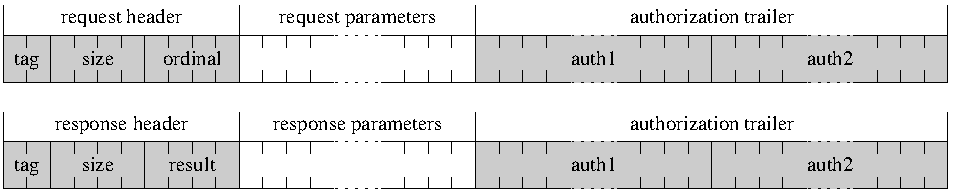
\includegraphics[height=24mm]{figures/tpm_command_structure}
		\caption{TPM command structure.}
		\label{fig:tpm_command}
	\end{center}
\end{figure}

\paragraph{Command Authorization.}
The purpose of several authorization protocols (e.g., OIAP and OSAP) is to
prove that the initiator of a command has permission to execute and to
access the involved data objects. For instance, they are used to establish
platform ownership, restrict key usage, and to apply access control to
(protected) objects. The proof comes from the knowledge of a shared secret,
the so called authorization data. The TPM treats knowledge of the corresponding
authorization data as a complete proof, i.e. no other checks are necessary.

% There are three protocols to proof the knowledge of a specific piece of authorization data. The
% \textit{Object-Independent Authorization Protocol} (OIAP) supports multiple authorization
% sessions for arbitrary entities whereby each entity has to be authorized individually.
% The \textit{Object-Specific Authorization Protocol} (OSAP) supports an authorization session
% for a single entity only, but has the advantage that the authorization data has to be used only
% once during the whole session. The \textit{ Delegate-Specific Authorization Protocol} (DSAP)
% supports the delegation of owner or entity authorization. New authorization information is inserted
% by the \textit{Authorization Data Insertion Protocol} (ADIP) during the creation of an entity. The
% \textit{Authorization Data Change Protocol} (ADCP) and the \textit{Asymmetric Authorization Change
% Protocol} (AACP) allow the changing of the authorization data for an entity.
%
% The protocols use a rolling nonce paradigm that is, they require that a nonce from one side is
% in use only for one message and its reply. For instance, a TPM's nonce which is returned as part
% of its command reply is part of the next command request. This mechanism is used to prevent
% reply as well as man-in-the-middle attacks.

%%%%%%%%%%%%%%%%%%%%%%%%%%%%%%%%%%%%%%%%%%%%%%%%%%%%%%%%%%%%%%%%%%%%%%%%%%%%%%%

\section{Design and Implementation}\label{sec:design}
The TPM emulator package comprises three main parts (see
Figure~\ref{fig:system_overview}): a user-space daemon (tpmd) that implements
the actual TPM emulator, a TPM device driver library (tddl) as the regular
interface to access the emulator, and a kernel module (tpmd\_dev) that
provides the character device \file{/dev/tpm} for low-level compatibility
with TPM device drivers.

\begin{figure}
	\begin{center}
		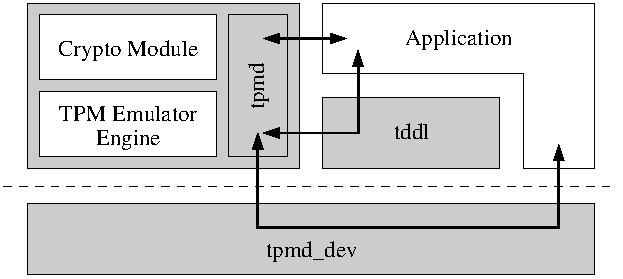
\includegraphics[width=.5\textwidth]{figures/system_overview}
		\caption{Overview of the TPM emulator package.}
		\label{fig:system_overview}
	\end{center}
\end{figure}

\subsection{TPM Device Driver Library and Kernel Module}
The most  convenient way to access a TPM is by means of the so-called TPM
Device Driver Library (TDDL) as specified by the TCG. The library provides
a simple and standardized interface for connecting to a TPM, querying its
state and capabilities as well as for sending TPM commands and receiving the
corresponding responses (for a comprehensive description of its functionality
we refer to the TSS specification~\cite{TSS}). Applications that use the
TDDL interface can be forced to use the TPM emulator instead of a real TPM
by simply exchanging this library. However, despite the existence of this
well defined and easy to use interface, several applications, tools, and
libraries rather directly access the TPM by its device driver interface, i.e.
by the device file \file{/dev/tpm}. Therefore, and in order to be compatible
with hardware TPMs at the lowest possible level, the TPM emulator package
includes a Linux kernel module called \texttt{tpmd\_dev}. This module
simulates a hardware TPM driver interface by providing the device
\file{/dev/tpm} and by forwarding all commands to the TPM emulator daemon.
This approach is completely transparent for an application and thus nearly
indistinguishable from the interaction with a real TPM.

\subsection{TPM Emulator Daemon}
The TPM emulator daemon implements the actual TPM emulator and consists of
the daemon application, the TPM emulator engine, and the cryptographic module.
After initializing the TPM emulator engine, the daemon application opens a
Unix domain socket and listens on it for incoming TPM commands. Upon the
reception of a valid command, the request is processed by the TPM emulator
engine and the corresponding response returned to the sender of the command.
Per default the socket name \file{/var/tpm/tpmd\_socket:0} is used but, if
required (e.g., if more than one TPM emulator instance has to be started),
an alternative name can be specified as a command-line argument.

\paragraph{TPM Emulator Engine.}
From a functional point of view, the TPM emulator engine is further divided
in the parameter (un)marshaling and (de)coding entity, the command execution
engine, the cryptographic engine and the key, data, and state storage entity.
Each part interacts with each other over a small set of well-defined functions.

The public API of the TPM emulator engine consists of only three functions.
The first function to be called is \func{tpm\_emulator\_init()} which
initializes the emulator. The function \func{tpm\_\-handle\_\-command()} can
then be used to execute an arbitrary number of TPM commands, before a call of
the function \func{tpm\_emulator\_shutdown()} shuts down the emulator.

\paragraph{Initialization and Self-Test.}
The initialization of the TPM emulator proceeds in three steps:
First, all data elements are set to their default values.
% The only exceptions are the \emph{disable}
% and \emph{deactivated} flags which are set to false although their default value is specified as
% true. This is done because starting the emulator can be seen as the users indication to use (i.e.,
% enable and activate) the TPM.
Next, an internal self-test of all cryptographic functions
is preformed. If one of the tests fails, the emulator goes into a fail-stop
mode and returns a corresponding error message on each command call. Finally,
if all tests succeeded, the emulator starts in the specified startup mode and
the remaining internal data is initialized accordingly. In the particular case
of startup mode \emph{save} this includes the restoration of all persistent
data from the persistent data storage file
(\file{/var/tpm/tpm\_emulator-1.2.x.y} as default).
Whenever the restoration of a previously stored state fails, the emulator
also switches to fail-stop mode.

\paragraph{Shutdown and Data Storage.}
On a regular shutdown, that is, if the emulator is not in fail-stop mode, all
persistent data is written into the persistent data storage file. Otherwise,
the internal state of the TPM emulator is discarded in order to avoid that
temporary malfunctions lead to a permanent failure of the emulator. Finally,
all allocated resources such as memory and file handles are released.

\paragraph{Command Execution}
The execution of a TPM command is initiated by calling the function
\func{tpm\_\-handle\_\-command()} with the marshaled TPM command (i.e., a
byte array) as input parameter. The command is then processed in three steps:
In the first step, the command is decoded into its three main components: the
request header, the command parameters, and the (optional) authorization
trailer (see Figure~\ref{fig:tpm_command}). After verifying whether the command
is allowed to be executed in the current state of the TPM, the input parameter
digest is computed and the parameters are further unmarshaled according to the
specific TPM command. The second step performs the actual execution of the
command and sets the command response parameters. If required, the
authorization trailer is verified in order to ensure command authorization
and integrity of the input parameters. In the last step, the response
authorization is computed and combined with the output parameters and the
response header. Finally, the response is marshaled into its byte
representation and returned to the caller.

\paragraph{Portability and System Independence.}
In order to facilitate the porting of the TPM emulator, the TPM emulator
engine contains no operating system or platform dependent functions (e.g.,
memory allocation and file handling), but accesses them by a set of predefined
functions. The actual implementation of these functions is in the
responsibility of the OS-dependent application. The therefore required API
as well as all system specific settings (e.g., whether the system uses
little- or big-endian byte ordering etc.) are specified in the header file
\file{tpm\_emulator\_config.h}.

Similar considerations lead to the separation and encapsulation of all
cryptographic functions. The TPM emulator accesses the required functionality,
i.e. the SHA-1, HMAC, random number generator, RSA, RC4, and multiple
precision integer arithmetic (bignum) methods by means of well defined
interfaces, but does not make any further assumptions regarding their
implementation. This allows for an easy replacement of individual function
blocks, e.g. in the case of (partly) available hardware support.

%%%%%%%%%%%%%%%%%%%%%%%%%%%%%%%%%%%%%%%%%%%%%%%%%%%%%%%%%%%%%%%%%%%%%%%%%%%%%%%

\section{Evaluation and Compliance Tests}\label{sec:state}
In order to investigate the scalability of our TPM emulator in relation to
the number of concurrently executed emulator instances on the same platform,
a number of TPM emulator daemons was started and a series of TPM command
executions was initiated on each instance in parallel. All experiments were
conducted on a IBM ThinkPad T43p (Pentium M @ 2\,GHz and 1\,GByte RAM) using
Linux kernel~2.6.19. The measured duration between sending the commands and
receiving all corresponding responses is shown in
Figure~\ref{plot:execution_time}. One can see that for light-weight
(Figure~\ref{plot:execution_time}(a)) as well as for computation-intensive
commands (Figure~\ref{plot:execution_time}(b)) the required time increases
linearly with the number of concurrently running emulator instances. This
shows that except for the unavoidable slowdown due to the availability of
only one single CPU, no significant overhead is introduced by concurrently
executing more than one emulator instance.

\marginpar{TODO: DAA on hardware TPM vs. emulator}

\begin{figure}
	\begin{center}
		\subfigure[TPM\_Extend]{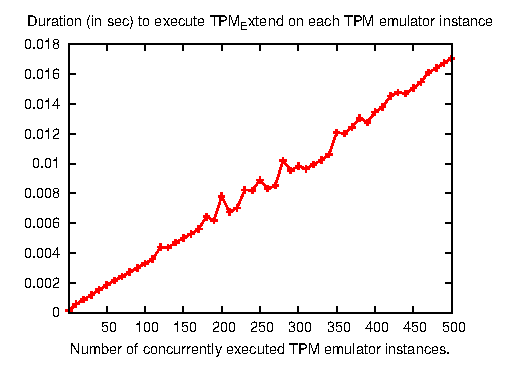
\includegraphics[width=.4\textwidth]{plots/duration_extend}}\quad%
		\subfigure[TPM\_SelfTest]{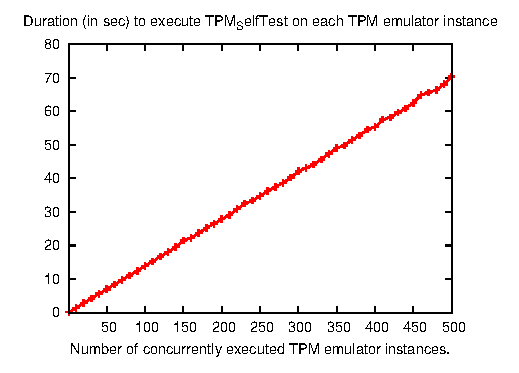
\includegraphics[width=.4\textwidth]{plots/duration_self_test}}
		\vspace*{-3mm}
		\caption{Duration for the execution of two commands on each TPM emulator
			instance.}
% The TPM command executions was initiated on each instance in parallel. One
% can observe that for light-weight (a) as well as computation-intensive commands (b) the required
% time increases linearly with the number of concurrently running emulator instances. This shows that
% except for the unavoidable slowdown due to the availability of only one single CPU, no significant
% overhead is introduced by concurrently running more than one emulator instance.}
		\label{plot:execution_time}
	\end{center}
\end{figure}

The results of several TPM compliance and functionality tests, in particular
those provided by TrouSerS~\cite{trousers} (package testsuite and package
tpm-tools), jTSS~\cite{jTSS} (package jTpmTools),
IBM DAA Test Suite~\cite{ibmdaatest} and
RUB/Sirrix~\cite{Sadeghi}, are summarized in Figure~\ref{plot:compliance}.
Note that, even though the emulator still lacks some functionality,
the most important and frequently used commands are already supported and
are compliant with the most recent TPM specification~\cite{TPM}.
A detailed list of the supported commands can be found in
Appendix~\ref{app:commands}.

\begin{figure}
	\begin{center}
		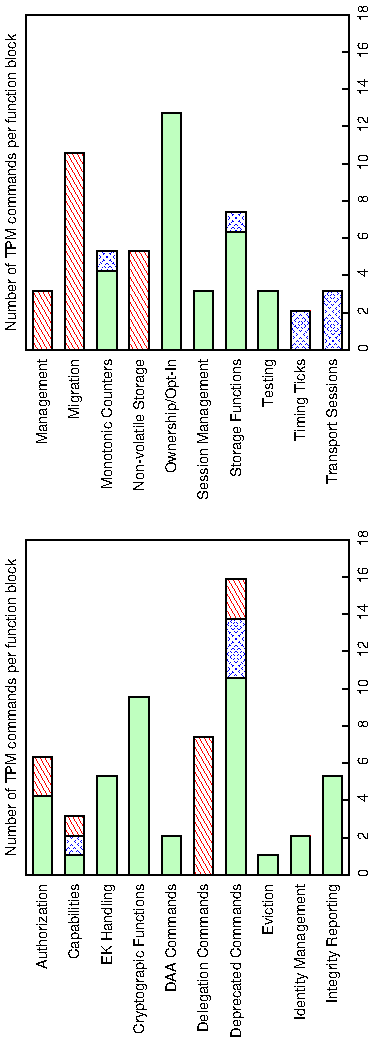
\includegraphics[angle=-90,scale=0.6]{plots/compliance}
		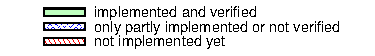
\includegraphics[origin=br,angle=90,scale=0.6]{plots/compliance_key}
		\caption{Summarized results of several TPM compliance and functionality
			tests.}
		\label{plot:compliance}
	\end{center}
\end{figure}

% \begin{table}[h]\footnotesize\centering
% \begin{tabular}{l|ccc}
% Function Block & \multicolumn{3}{c}{Number of TPM commands} \\
%                & Total & Implemented & Verified \\ \hline
% Auditing               &  3 &  3 &  3 \\
% Authorization          &  6 &  4 &  4 \\
% Capabilities           &  3 &  2 &  1 \\
% Credential Handling    &  6 &  6 &  6 \\
% Cryptograpic Functions &  9 &  9 &  9 \\
% DAA Commands           &  2 &  2 &  2 \\
% Delegation Commands    &  7 &  0 &  0 \\
% Deprecated Commands    & 13 & 11 &  8 \\
% Eviction               &  1 &  1 &  1 \\
% Identity Management    &  2 &  2 &  2 \\
% Integrity Reporting    &  5 &  5 &  5 \\
% \end{tabular}\hspace*{10mm}
% \begin{tabular}{l|ccc}
% Function Block & \multicolumn{3}{c}{Number of TPM commands} \\
%                & Total & Implemented & Verified \\ \hline
% Maintenance            &  5 &  0 &  0 \\
% Management             &  3 &  0 &  0 \\
% Migration              & 10 &  0 &  0 \\
% Monotonic Counters     &  5 &  5 &  0 \\
% Non-volatile Storage   &  5 &  0 &  0 \\
% Ownership/Opt-In       & 12 & 12 & 12 \\
% Session Management     &  3 &  3 &  3 \\
% Storage Functions      &  8 &  7 &  7 \\
% Testing                &  3 &  3 &  3 \\
% Timing Ticks           &  3 &  3 &  0 \\
% Transport Sessions     &  3 &  3 &  0 \\
% \end{tabular}
% \caption{Summarized results of several TPM compliance and functionality tests.}
% \label{tab:compliance}
% \end{table}

%%%%%%%%%%%%%%%%%%%%%%%%%%%%%%%%%%%%%%%%%%%%%%%%%%%%%%%%%%%%%%%%%%%%%%%%%%%%%%%

\section{Conclusions and Future Work}\label{sec:conclusion}
In this paper, we presented a software-based TPM emulator for Unix. Even
though the emulator still lacks some functionality, it is compatible with
the most relevant software tools and works very well with almost all
available TPM-enabled Unix applications. In fact, the most important and
frequently used commands are already supported. We showed that hundreds of
(concurrently running) emulator instances can be efficiently simulated on
a single platform, allowing for the implementation of low-cost test-beds
and simulators. In addition, the emulator provides programmers of trusted
computing systems with a powerful testing and debugging tool that can also
be used for training and educational purposes.
The emulator is still a work in progress and our future attention will
focus the completion of the missing commands. A further step is the portage
of the TPM emulator package to Windows and Mac~OS~X operating systems.

%%\bibliographystyle{plain}
%%\bibliography{biblio}

\begin{thebibliography}{10}

\bibitem{Aaraj}
Najwa Aaraj, Anand Raghunathan, Srivaths Ravi, and Niraj~K. Jha.
\newblock {Energy and Execution Time Analysis of a Software-Based Trusted
  Platform Module}.
\newblock In {\em Proceedings of the Conference on Design, Automation and Test
  in Europe (DATE '07)}, pp. 1128--1133, 2007.

\bibitem{Xen}
Melvin~J. Anderson, Micha Moffie, and Chris~I. Dalton.
\newblock {Towards Trustworthy Virtualisation Environments: Xen Library OS
  Security Service Infrastructure}.
\newblock Technical Report HPL-2007-69, HP Laboratories Bristol, April 2007.

\bibitem{Bishop2003}
Matt Bishop.
\newblock {\em {Computer Security: Art and Science}}.
\newblock Addison Wesley, 2003.

%\bibitem{GMP}
%Torbj{\"o}rn Granlund et~al.
%\newblock {GNU Multiple Precision Arithmetic Library}.
%\newblock \newline\url{http://gmplib.org/}.

\bibitem{Mitchell2005}
Chris Mitchell et~al.
\newblock {\em {Trusted Computing}}.
\newblock IET, 2005.

\bibitem{Sadeghi}
Ahmad-Reza Sadeghi, Marcel Selhorst, Christian St\"{u}ble, Christian Wachsmann,
  and Marcel Winandy.
\newblock {TCG inside?: A Note on TPM Specification Compliance}.
\newblock In {\em Proceedings of the 1st ACM Workshop on Scalable Trusted
  Computing (STC '06)}, pp. 47--56, 2006.

\bibitem{Sarmenta}
Luis F.~G. Sarmenta, Marten van Dijk, Charles~W. O'Donnell, Jonathan Rhodes,
  and Srinivas Devadas.
\newblock {Virtual monotonic counters and count-limited objects using a TPM
  without a trusted OS}.
\newblock In {\em Proceedings of the 1st ACM Workshop on Scalable Trusted
  Computing (STC '06)}, pp. 27--42, 2006.

\bibitem{TPMEmu}
Mario Strasser et~al.
\newblock {Software-based TPM Emulator for Linux}.
\newblock \newline\url{http://developer.berlios.de/projects/tpm-emulator}.

\bibitem{TCGArch}
{Trusted Computing Group}.
\newblock {Architecture Overview}.

\bibitem{TSS}
{Trusted Computing Group}.
\newblock {TPM Software Stack (TSS) Specification, Version 1.2}.
\newblock \newline\url{https://www.trustedcomputinggroup.org/specs/TSS/}.

\bibitem{TPM}
{Trusted Computing Group}.
\newblock {TPM Specification, Version 1.2, Revision 103}.
\newblock \newline\url{https://www.trustedcomputinggroup.org/specs/TPM}.

\bibitem{jTSS}
{TU Graz, IAIK}.
\newblock {jTSS -- Java TCG Software Stack}.
\newblock \newline\url{http://trustedjava.sourceforge.net/}.

\bibitem{trousers}
Kent Yoder et~al.
\newblock {TrouSerS -- Open-source TCG Software Stack}.
\newblock \newline\url{http://trousers.sourceforge.net/}.

\bibitem{ibmdaatest}
Roger Zimmermann.
\newblock {IBM Direct Anonymous Attestation Tools -- TPM Test Suite}.
\newblock
  \newline\url{http://www.zurich.ibm.com/security/daa/IBM-DAA-TPM-TestSuite-Ov%
erview.html}.

\end{thebibliography}

\appendix
\newpage

\section{Supported TPM Commands}\label{app:commands}
\definecolor{tpmgray}{gray}{0.85}
\newcommand{\tpmred}{tpmgray!10!red!50!white}
\newcommand{\tpmyellow}{tpmgray!10!yellow!50!white}
\newcommand{\tpmgreen}{tpmgray!10!green!50!white}
\newcommand{\tpmcolor}{tpmgray}

\newcommand{\tpmcmd}[6]{
	\begin{tabular}{p{4.5cm}|p{0.35cm}|p{0.4cm}|p{0.25cm}|p{2.5cm}|p{2cm}}
		\rowcolor{\tpmcolor}
			{\scriptsize\textsf{#1}} &
			{\scriptsize\textsf{#2}} &
			{\scriptsize\makebox[0.4cm][r]{#3}} &
			{\scriptsize\makebox[0.25cm][c]{#4}} &
			{\scriptsize\texttt{#5}} &
			{\scriptsize #6}\\
	\end{tabular}
}
\newcommand{\tpmcmdr}[6]{
	\renewcommand{\tpmcolor}{\tpmred}
	\tpmcmd{#1}{#2}{#3}{#4}{#5}{#6}
	\renewcommand{\tpmcolor}{tpmgray}
}
\newcommand{\tpmcmdg}[6]{
	\renewcommand{\tpmcolor}{\tpmgreen}
	\tpmcmd{#1}{#2}{#3}{#4}{#5}{#6}
	\renewcommand{\tpmcolor}{tpmgray}
}
\newcommand{\tpmcmdy}[6]{
	\renewcommand{\tpmcolor}{\tpmyellow}
	\tpmcmd{#1}{#2}{#3}{#4}{#5}{#6}
	\renewcommand{\tpmcolor}{tpmgray}
}
The following table shows the current state of implementation for each
command from the most recent TPM specification~\cite{TPM}. The background
color of each row corresponds to the states:
\colorbox{\tpmgreen}{\emph{completed}},
\colorbox{\tpmyellow}{\emph{partially implemented}}, or
\colorbox{\tpmred}{\emph{missing}}.

Each row contains several information about the command:
the name;
the version of the TPM specification, where the command was defined at first;
the ordinal;
a letter indicating, whether the command is mandatory (M), optional (O),
deprecated (D), or removed (X);
the source file, where the command is implemented;
and some space for additional notes.
These notes include the result of the performed compliance tests and the
percentage of work to do, if the command is not yet or only partially
implemented.


\begin{enumerate}
	\item Admin Startup and State (pp. 5--10)\\
\tpmcmdg{TPM\_Init}{1.1}{151}{M}{tpm\_startup.c}{}\\
\tpmcmdg{TPM\_Startup}{1.1}{153}{M}{tpm\_startup.c}{}\\
\tpmcmdg{TPM\_SaveState}{1.1}{152}{M}{tpm\_startup.c}{}
	\item Admin Testing (pp. 11--14)\\
\tpmcmdg{TPM\_SelfTestFull}{1.1}{80}{M}{tpm\_testing.c}{passed \cite{trousers,jTSS}}\\
\tpmcmdg{TPM\_ContinueSelfTest}{1.1}{83}{M}{tpm\_testing.c}{}\\
\tpmcmdg{TPM\_GetTestResult}{1.1}{84}{M}{tpm\_testing.c}{passed \cite{trousers,jTSS}}
	\item Admin Opt-in (pp. 15--22)\\
\tpmcmdg{TPM\_SetOwnerInstall}{1.1}{113}{M}{tpm\_owner.c}{}\\
\tpmcmdg{TPM\_OwnerSetDisable}{1.1}{110}{M}{tpm\_owner.c}{}\\
\tpmcmdg{TPM\_PhysicalEnable}{1.1}{111}{M}{tpm\_owner.c}{}\\
\tpmcmdg{TPM\_PhysicalDisable}{1.1}{112}{M}{tpm\_owner.c}{}\\
\tpmcmdg{TPM\_PhysicalSetDeactivated}{1.1}{114}{M}{tpm\_owner.c}{}\\
\tpmcmdg{TPM\_SetTempDeactivated}{1.1}{115}{M}{tpm\_owner.c}{}\\
\tpmcmdg{TPM\_SetOperatorAuth}{1.2}{116}{M}{tpm\_owner.c}{}
	\item Admin Ownership (pp. 23--36)\\
\tpmcmdg{TPM\_TakeOwnership}{1.1}{13}{M}{tpm\_owner.c}{passed \cite{trousers,jTSS}}\\
\tpmcmdg{TPM\_OwnerClear}{1.1}{91}{M}{tpm\_owner.c}{}\\
\tpmcmdg{TPM\_ForceClear}{1.1}{93}{M}{tpm\_owner.c}{}\\
\tpmcmdg{TPM\_DisableOwnerClear}{1.1}{92}{M}{tpm\_owner.c}{}\\
\tpmcmdg{TPM\_DisableForceClear}{1.1}{94}{M}{tpm\_owner.c}{}\\
\tpmcmdg{TSC\_PhysicalPresence}{1.1}{}{M}{tpm\_owner.c}{}\\
\tpmcmdg{TSC\_ResetEstablishmentBit}{1.2}{}{M}{tpm\_owner.c}{}
	\item Capability Commands (pp. 37--42)\\
\tpmcmdy{TPM\_GetCapability}{1.1}{101}{M}{tpm\_capability.c}{TODO: 45\,\%}\\
\tpmcmdr{TPM\_SetCapability}{1.2}{63}{M}{tpm\_capability.c}{TODO: 100\,\%}\\
\tpmcmdg{TPM\_GetCapabilityOwner}{1.1}{102}{M}{tpm\_capability.c}{}
	\item Auditing (pp. 43--51)\\
\tpmcmdg{TPM\_GetAuditDigest}{1.2}{133}{O}{tpm\_audit.c}{}\\
\tpmcmdg{TPM\_GetAuditDigestSigned}{1.2}{134}{O}{tpm\_audit.c}{}\\
\tpmcmdg{TPM\_SetOrdinalAuditStatus}{1.1}{141}{O}{tpm\_.auditc}{}
	\item Administrative Functions -- Management (pp. 52--57)\\
\tpmcmdr{TPM\_FieldUpgrade}{1.1}{170}{O}{tpm\_management.c}{TODO: 100\,\%}\\
\tpmcmdr{TPM\_SetRedirection}{1.1}{154}{O}{tpm\_management.c}{TODO: 100\,\%}\\
\tpmcmdr{TPM\_ResetLockValue}{1.2}{64}{M}{tpm\_management.c}{TODO: 100\,\%}
	\item Storage Functions (pp. 58--81)\\
\tpmcmdg{TPM\_Seal}{1.1}{23}{M}{tpm\_storage.c}{passed \cite{trousers,jTSS,Sadeghi}}\\
\tpmcmdg{TPM\_Unseal}{1.1}{24}{M}{tpm\_storage.c}{passed \cite{jTSS}}\\
\tpmcmdg{TPM\_UnBind}{1.1}{30}{M}{tpm\_storage.c}{passed \cite{trousers,jTSS,Sadeghi}}\\
\tpmcmdg{TPM\_CreateWrapKey}{1.1}{31}{M}{tpm\_storage.c}{passed \cite{trousers,jTSS,Sadeghi}}\\
\tpmcmdy{TPM\_LoadKey2}{1.2}{65}{M}{tpm\_storage.c}{emulated by 32}\\
\tpmcmdg{TPM\_GetPubKey}{1.1}{33}{M}{tpm\_storage.c}{passed \cite{trousers}}\\
\tpmcmdr{TPM\_Sealx}{1.2}{61}{O}{tpm\_storage.c}{TODO: 100\,\%}
	\item Migration (pp. 82--108)\\
\tpmcmdr{TPM\_CreateMigrationBlob}{1.1}{40}{M}{tpm\_migration.c}{TODO: 100\,\%}\\
\tpmcmdr{TPM\_ConvertMigrationBlob}{1.1}{42}{M}{tpm\_migration.c}{TODO: 100\,\%}\\
\tpmcmdr{TPM\_AuthorizeMigrationKey}{1.1}{43}{M}{tpm\_migration.c}{TODO: 100\,\%}\\
\tpmcmdr{TPM\_MigrateKey}{1.2}{37}{M}{tpm\_migration.c}{TODO: 100\,\%}\\
\tpmcmdr{TPM\_CMK\_SetRestrictions}{1.2}{28}{M}{tpm\_migration.c}{TODO: 100\,\%}\\
\tpmcmdr{TPM\_CMK\_ApproveMA}{1.2}{29}{M}{tpm\_migration.c}{TODO: 100\,\%}\\
\tpmcmdr{TPM\_CMK\_CreateKey}{1.2}{19}{M}{tpm\_migration.c}{TODO: 100\,\%}\\
\tpmcmdr{TPM\_CMK\_CreateTicket}{1.2}{18}{M}{tpm\_migration.c}{TODO: 100\,\%}\\
\tpmcmdr{TPM\_CMK\_CreateBlob}{1.2}{27}{M}{tpm\_migration.c}{TODO: 100\,\%}\\
\tpmcmdr{TPM\_CMK\_ConvertMigration}{1.2}{36}{M}{tpm\_migration.c}{TODO: 100\,\%}
	\item Maintenance Functions (optional, pp. 109--118)\\
\tpmcmdr{TPM\_CreateMaintenanceArchive}{1.1}{44}{O}{tpm\_maintenance.c}{TODO: 100\,\%}\\
\tpmcmdr{TPM\_LoadMaintenanceArchive}{1.1}{45}{O}{tpm\_maintenance.c}{TODO: 100\,\%}\\
\tpmcmdr{TPM\_KillMaintenanceFeature}{1.1}{46}{O}{tpm\_maintenance.c}{TODO: 100\,\%}\\
\tpmcmdr{TPM\_LoadManuMaintPub}{1.1}{47}{O}{tpm\_maintenance.c}{TODO: 100\,\%}\\
\tpmcmdr{TPM\_ReadManuMaintPub}{1.1}{48}{O}{tpm\_maintenance.c}{TODO: 100\,\%}
	\item Cryptographic Functions (pp. 119--136)\\
\tpmcmdg{TPM\_SHA1Start}{1.1}{160}{M}{tpm\_crypto.c}{passed \cite{trousers,jTSS}}\\
\tpmcmdg{TPM\_SHA1Update}{1.1}{161}{M}{tpm\_crypto.c}{passed \cite{trousers,jTSS}}\\
\tpmcmdg{TPM\_SHA1Complete}{1.1}{162}{M}{tpm\_crypto.c}{passed \cite{trousers,jTSS}}\\
\tpmcmdg{TPM\_SHA1CompleteExtend}{1.1}{163}{M}{tpm\_crypto.c}{passed \cite{trousers}}\\
\tpmcmdg{TPM\_Sign}{1.1}{60}{M}{tpm\_crypto.c}{passed \cite{trousers,jTSS,Sadeghi}}\\
\tpmcmdg{TPM\_GetRandom}{1.1}{70}{M}{tpm\_crypto.c}{passed \cite{trousers,jTSS,Sadeghi}}\\
\tpmcmdg{TPM\_StirRandom}{1.1}{71}{M}{tpm\_crypto.c}{passed \cite{trousers,jTSS}}\\
\tpmcmdg{TPM\_CertifyKey}{1.1}{50}{M}{tpm\_crypto.c}{passed \cite{trousers,jTSS}}\\
\tpmcmdg{TPM\_CertifyKey2}{1.2}{51}{M}{tpm\_crypto.c}{}
	\item Endorsement Key Handling (pp. 137--145)\\
\tpmcmdy{TPM\_CreateEndorsementKeyPair}{1.1}{120}{M}{tpm\_credentials.c}{disabled}\\
\tpmcmdg{TPM\_CreateRevocableEK}{1.2}{127}{O}{tpm\_credentials.c}{}\\
\tpmcmdg{TPM\_RevokeTrust}{1.2}{128}{O}{tpm\_credentials.c}{}\\
\tpmcmdg{TPM\_ReadPubek}{1.1}{124}{M}{tpm\_credentials.c}{passed \cite{trousers,jTSS}}\\
\tpmcmdg{TPM\_OwnerReadInternalPub}{1.2}{129}{M}{tpm\_credentials.c}{}
	\item Identity Creation and Activation (pp. 146--152)\\
\tpmcmdg{TPM\_MakeIdentity}{1.1}{121}{M}{tpm\_identity.c}{passed \cite{trousers,jTSS}}\\
\tpmcmdg{TPM\_ActivateIdentity}{1.1}{122}{M}{tpm\_identity.c}{passed \cite{trousers,jTSS}}
	\item Integrity Collection and Reporting (pp. 153--163)\\
\tpmcmdg{TPM\_Extend}{1.1}{20}{M}{tpm\_integrity.c}{passed \cite{trousers,jTSS}}\\
\tpmcmdg{TPM\_PCRRead}{1.1}{21}{M}{tpm\_integrity.c}{passed \cite{trousers,jTSS,Sadeghi}}\\
\tpmcmdg{TPM\_Quote}{1.1}{22}{M}{tpm\_integrity.c}{passed \cite{trousers,jTSS}}\\
\tpmcmdg{TPM\_PCR\_Reset}{1.2}{200}{M}{tpm\_integrity.c}{no support \cite{jTSS}}\\
\tpmcmdg{TPM\_Quote2}{1.2}{62}{M}{tpm\_integrity.c}{no support \cite{jTSS}}
	\item Changing AuthData (pp. 164--168)\\
\tpmcmdg{TPM\_ChangeAuth}{1.1}{12}{M}{tpm\_authorization.c}{passed \cite{trousers}}\\
\tpmcmdg{TPM\_ChangeAuthOwner}{1.1}{16}{M}{tpm\_authorization.c}{}
	\item Authorization Sessions (pp. 169--181)\\
\tpmcmdg{TPM\_OIAP}{1.1}{10}{M}{tpm\_authorization.c}{not random \cite{Sadeghi}}\\
\tpmcmdg{TPM\_OSAP}{1.1}{11}{M}{tpm\_authorization.c}{not random \cite{Sadeghi}}\\
\tpmcmdr{TPM\_DSAP}{1.2}{17}{M}{tpm\_authorization.c}{TODO: 100\,\%}\\
\tpmcmdy{TPM\_SetOwnerPointer}{1.2}{117}{M}{tpm\_authorization.c}{disabled}
	\item Delegation Commands (pp. 182--201)\\
\tpmcmdr{TPM\_Delegate\_Manage}{1.2}{210}{M}{tpm\_delegation.c}{TODO: 100\,\%}\\
\tpmcmdr{TPM\_Delegate\_CreateKeyDelegation}{1.2}{212}{M}{tpm\_delegation.c}{TODO: 100\,\%}\\
\tpmcmdr{TPM\_Delegate\_CreateOwnerDelegation}{1.2}{213}{M}{tpm\_delegation.c}{TODO: 100\,\%}\\
\tpmcmdr{TPM\_Delegate\_LoadOwnerDelegation}{1.2}{216}{M}{tpm\_delegation.c}{TODO: 100\,\%}\\
\tpmcmdr{TPM\_Delegate\_ReadTable}{1.2}{219}{M}{tpm\_delegation.c}{TODO: 100\,\%}\\
\tpmcmdr{TPM\_Delegate\_UpdateVerification}{1.2}{209}{M}{tpm\_delegation.c}{TODO: 100\,\%}\\
\tpmcmdr{TPM\_Delegate\_VerifyDelegation}{1.2}{214}{M}{tpm\_delegation.c}{TODO: 100\,\%}
	\item Non-volatile Storage (pp. 202--215)\\
\tpmcmdr{TPM\_NV\_DefineSpace}{1.2}{204}{M}{tpm\_nv\_storage.c}{TODO: 100\,\%}\\
\tpmcmdr{TPM\_NV\_WriteValue}{1.2}{205}{M}{tpm\_nv\_storage.c}{TODO: 100\,\%}\\
\tpmcmdr{TPM\_NV\_WriteValueAuth}{1.2}{206}{M}{tpm\_nv\_storage.c}{TODO: 100\,\%}\\
\tpmcmdr{TPM\_NV\_ReadValue}{1.2}{207}{M}{tpm\_nv\_storage.c}{TODO: 100\,\%}\\
\tpmcmdr{TPM\_NV\_ReadValueAuth}{1.2}{208}{M}{tpm\_nv\_storage.c}{TODO: 100\,\%}
	\item Session Management (pp. 216--223)\\
\tpmcmdg{TPM\_KeyControlOwner}{1.2}{35}{M}{tpm\_context.c}{}\\
\tpmcmdg{TPM\_SaveContext}{1.2}{184}{M}{tpm\_context.c}{}\\
\tpmcmdg{TPM\_LoadContext}{1.2}{185}{M}{tpm\_context.c}{}
	\item Eviction (pp. 224--226)\\
\tpmcmdy{TPM\_FlushSpecific}{1.2}{186}{M}{tpm\_eviction.c}{TODO: 75\,\%}
	\item Timing Ticks (pp. 227--230)\\
\tpmcmdg{TPM\_GetTicks}{1.2}{241}{M}{tpm\_ticks.c}{no support \cite{jTSS}}\\
\tpmcmdg{TPM\_TickStampBlob}{1.2}{242}{M}{tpm\_ticks.c}{no support \cite{jTSS}}
	\item Transport Sessions (pp. 231--244)\\
\tpmcmdg{TPM\_EstablishTransport}{1.2}{230}{M}{tpm\_transport.c}{}\\
\tpmcmdg{TPM\_ExecuteTransport}{1.2}{231}{M}{tpm\_transport.c}{}\\
\tpmcmdg{TPM\_ReleaseTransportSigned}{1.2}{232}{M}{tpm\_transport.c}{}
	\item Monotonic Counter (pp. 245--254)\\
\tpmcmdg{TPM\_CreateCounter}{1.2}{220}{M}{tpm\_counter.c}{}\\
\tpmcmdg{TPM\_IncrementCounter}{1.2}{221}{M}{tpm\_counter.c}{}\\
\tpmcmdg{TPM\_ReadCounter}{1.2}{222}{M}{tpm\_counter.c}{}\\
\tpmcmdg{TPM\_ReleaseCounter}{1.2}{223}{M}{tpm\_counter.c}{}\\
\tpmcmdg{TPM\_ReleaseCounterOwner}{1.2}{224}{M}{tpm\_counter.c}{}
	\item DAA Commands (pp. 255--282)\\
\tpmcmdg{TPM\_Join}{1.2}{41}{M}{tpm\_daa.c}{passed \cite{ibmdaatest}}\\
\tpmcmdg{TPM\_Sign}{1.2}{49}{M}{tpm\_daa.c}{passed \cite{ibmdaatest}}
	\item Deprecated Commands (pp. 283--309)\\
\tpmcmdg{TPM\_EvictKey}{1.1}{34}{D}{tpm\_deprecated.c}{}\\
\tpmcmdg{TPM\_Terminate\_Handle}{1.1}{150}{D}{tpm\_deprecated.c}{}\\
\tpmcmdg{TPM\_SaveKeyContext}{1.1}{180}{D}{tpm\_deprecated.c}{}\\
\tpmcmdg{TPM\_LoadKeyContext}{1.1}{181}{D}{tpm\_deprecated.c}{}\\
\tpmcmdg{TPM\_SaveAuthContext}{1.1}{182}{D}{tpm\_deprecated.c}{}\\
\tpmcmdg{TPM\_LoadAuthContext}{1.1}{183}{D}{tpm\_deprecated.c}{}\\
\tpmcmdg{TPM\_DirWriteAuth}{1.1}{25}{D}{tpm\_deprecated.c}{passed \cite{trousers,jTSS}}\\
\tpmcmdg{TPM\_DirRead}{1.1}{26}{D}{tpm\_deprecated.c}{passed \cite{trousers,jTSS}}\\
\tpmcmdr{TPM\_ChangeAuthAsymStart}{1.1}{14}{D}{tpm\_deprecated.c}{TODO: 95\,\%}\\
\tpmcmdr{TPM\_ChangeAuthAsymFinish}{1.1}{15}{D}{tpm\_deprecated.c}{TODO: 100\,\%}\\
\tpmcmdg{TPM\_Reset}{1.1}{90}{D}{tpm\_deprecated.c}{}\\
\tpmcmdg{TPM\_OwnerReadPubek}{1.1}{125}{D}{tpm\_deprecated.c}{}\\
\tpmcmdg{TPM\_DisablePubekRead}{1.1}{126}{?}{tpm\_credentials.c}{spec error?}\\
\tpmcmdg{TPM\_LoadKey}{1.1b}{32}{D}{tpm\_storage.c}{passed \cite{trousers,jTSS}}
	\item Deleted Commands (pp. 310--314)\\
\tpmcmdr{TPM\_GetCapabilitySigned}{1.1}{100}{X}{}{}\\
\tpmcmdr{TPM\_GetOrdinalAuditStatus}{1.1}{140}{X}{}{}\\
\tpmcmdg{TPM\_CertifySelfTest}{1.1}{82}{X}{tpm\_deprecated.c}{bad ordinal~\cite{trousers}}\\
\tpmcmdr{TPM\_GetAuditEventSigned}{1.1}{130}{X}{}{}\\
\tpmcmdr{TPM\_GetAuditEventSigned}{1.1}{131}{X}{}{}
\end{enumerate}
\end{document}
